\chapter{Resultados}


\section{Estudio sobre la influencia de marcadores en el declive cognitivo en la Enfermedad de Parkinson}

Como resultado de la realización del algoritmo anterior, se obtuvieron las dos tablas siguientes, con las que se realizará un estudio de las variables:

\begin{description}
	\item{\textbf{Tabla 1:}} comparativa de las características clínicas y demográficas entre pacientes PD y el grupo de control en la linea de base.
	
	En la tabla \ref{tab:tabla3}, se observa como para cada grupo se muestra, en el caso de las variables cualitativas, el valor medio de sujetos y mujeres y su porcentaje en comparación con el total; y en el caso de las características cuantitativa, la media, la desviación típica y los máximos y mínimos. Además, se marca con una \textit{a} en la columna 'post-hoc' cuales de ellas son indicativas del declive cognitivo al inicio del estudio.
	
	
	\begin{table}[t]
		\begin{adjustbox}{width=\textwidth}
			\begin{tabular}{|l||c|c|c|}
				\toprule
				Group &                                 PD &                                 HC & Post-hoc \\
				\midrule
				Subjects &                        423 (61.9\%) &                        196 (28.7\%) &    -      \\
				Female &                        146 (34.5\%) &                         70 (35.7\%) &  -    \\
				APOE4 &                  101 (26.3\%) n=384 &                   47 (26.4\%) n=178 &   -   \\
				Age &            61.7 (9.7) (33.5, 84.9) &           60.8 (11.2) (30.6, 83.7) &  -    \\
				Education &         15.56 (2.97) (5.00, 26.00) &         16.04 (2.89) (8.00, 24.00) &   -   \\
				\hline
				GDS &          2.32 (2.44) (0.00, 14.00) &          1.29 (2.10) (0.00, 15.00) &        a \\
				UPSIT &         22.35 (8.23) (1.00, 40.00) &        33.98 (4.86) (11.00, 40.00) &        a \\
				REM &          4.12 (2.69) (0.00, 12.00) &          2.83 (2.26) (0.00, 11.00) &        a \\
				UPDRS3 &         20.89 (8.85) (4.00, 51.00) &          1.21 (2.19) (0.00, 13.00) &        a \\
				\hline
				\multicolumn{4}{ |l| }{Cognitive outcomes} \\
				\hline
				MOCA &        27.13 (2.32) (17.00, 30.00) &        28.23 (1.11) (26.00, 30.00) &        a \\
				LNS &         10.59 (2.66) (2.00, 20.00) &         10.87 (2.57) (2.00, 20.00) &   -   \\
				SDMT &         41.18 (9.73) (7.00, 82.00) &       46.77 (10.53) (20.00, 83.00) &        a \\
				JLO &         12.77 (2.13) (5.00, 15.00) &         13.12 (1.98) (4.00, 15.00) &  -    \\
				INMEDIATE &         24.44 (4.98) (9.00, 36.00) &        26.05 (4.50) (15.00, 35.00) &        a \\
				HVLTRDLY &          8.36 (2.52) (0.00, 12.00) &          9.29 (2.32) (2.00, 12.00) &        a \\
				SFT &      48.67 (11.63) (20.00, 103.00) &       51.80 (11.20) (22.00, 80.00) &        a \\
				ADL &       93.14 (5.89) (70.00, 100.00) &      100.00 (0.00) (100.00, 100.00) &  -    \\
				SCOPA &          9.51 (6.18) (0.00, 39.00) &          5.83 (3.69) (0.00, 20.00) &        a \\
				\hline
				\multicolumn{4}{ |l| }{CSF and DAT imaging markers} \\
				\hline
				ABETA &  909.55 (410.73) (238.80, 3707.00) & 1019.37 (499.46) (239.10, 3297.00) &        a \\
				ASYN & 1506.70 (666.59) (432.40, 5256.90) & 1695.19 (747.42) (488.60, 4683.10) &        a \\
				TAU &     169.54 (56.80) (80.93, 467.00) &     191.64 (79.26) (81.96, 580.80) &        a \\
				PTAU &         14.87 (5.25) (8.01, 40.13) &         17.52 (8.35) (8.08, 73.61) &        a \\
				pTauAB &           0.02 (0.01) (0.01, 0.08) &           0.02 (0.02) (0.01, 0.18) &  -    \\
				MEANPUT &           0.83 (0.30) (0.24, 2.17) &           2.15 (0.56) (0.64, 3.89) &        a \\
				MEANCAU &           2.00 (0.56) (0.39, 3.71) &           2.98 (0.63) (1.32, 5.20) &        a \\
				\bottomrule
			\end{tabular}
		\end{adjustbox}
		\caption{Características clínicas y demográficas del grupo de pacientes (PD) y del grupo de control (HC) al inicio del estudio.}
		\label{tab:tabla3}
	\end{table}
	
	
	
	
	\item{\textbf{Tabla 2:}} comparativa entre la evolución de los pacientes con Parkinson a los distintos grupos de avance de la enfermedad (PD\_CU, PD\_MCI y PDD) al inicio del estudio.
	
	En la tabla \ref{tab:tabla2}, se realizan los mismos cálculos estadísticos de la tabla \ref{tab:tabla3}, ya que permiten visualizar la influencia de los distintos parámetros en la evolución de los tres grupos expuestos. Con las columnas 'p-value' y 'post-hoc' se reflejan las variables que son significativas para predecir el avance de la enfermedad a cada uno de los grupos y que permitirían pronosticar si el paciente puede desarrollar deterioro cognitivo medio o demencia en las primeras fases de la enfermedad.
	
	\begin{table}[t]
		\begin{adjustbox}{width=\textwidth}
			\begin{tabular}{|l||c|c|c|c|c|}
				\toprule
				Group &                              PD\_CU &                             PD\_MCI &                        PDD &   p-value & Post-hoc \\ 
				\midrule
				Subjects &                        323 (47.3\%) &                         83 (12.2\%) &                          17 (2.5\%) &     -      &    -      \\
				Female &                        120 (37.2\%) &                         20 (24.1\%) &                          6 (35.3\%) &     0.083 &  -    \\
				APOE4 &                   78 (26.4\%) n=295 &                    18 (23.7\%) n=76 &                     5 (38.5\%) n=13 &     0.101 &  -    \\
				Age &            60.1 (9.8) (33.5, 82.3) &            66.0 (7.4) (48.0, 84.9) &            69.4 (7.4) (54.8, 83.0) & $<$ 0.001 &      a,b \\
				Education &         15.70 (2.87) (8.00, 26.00) &         14.99 (2.82) (8.00, 21.00) &         15.59 (4.91) (5.00, 21.00) &     0.150 &  -    \\
				\hline
				GDS &          2.17 (2.40) (0.00, 14.00) &          2.86 (2.61) (0.00, 13.00) &           2.71 (2.11) (0.00, 8.00) &     0.058 &   -   \\
				UPSIT &         23.41 (7.87) (5.00, 39.00) &         19.54 (8.60) (1.00, 40.00) &         16.06 (7.39) (5.00, 31.00) & $<$ 0.001 &      a,b \\
				REM &          3.82 (2.54) (0.00, 12.00) &          5.06 (2.90) (0.00, 12.00) &          5.24 (3.11) (0.00, 12.00) & $<$ 0.001 &        a \\
				UPDRS3 &         20.51 (8.73) (5.00, 47.00) &         22.29 (9.40) (4.00, 51.00) &        21.29 (8.18) (10.00, 39.00) &     0.260 &  -    \\
				\hline
				\multicolumn{6}{|l|}{Cognitive outcomes} \\
				\hline
				MOCA &        27.33 (2.17) (19.00, 30.00) &        26.58 (2.70) (17.00, 30.00) &        25.94 (2.38) (21.00, 29.00) &     0.003 &    -      \\
				LNS &         11.04 (2.50) (2.00, 20.00) &          9.29 (2.58) (4.00, 17.00) &          8.29 (2.78) (3.00, 13.00) & $<$ 0.001 &      a,b \\
				SDMT &        42.94 (8.75) (17.00, 82.00) &        36.69 (10.18) (7.00, 58.00) &       29.82 (10.85) (15.00, 50.00) & $<$ 0.001 &      a,b \\
				JLO &         12.98 (1.96) (5.00, 15.00) &         12.19 (2.44) (6.00, 15.00) &         11.53 (2.67) (6.00, 15.00) & $<$ 0.001 &        a \\
				INMEDIATE &         25.26 (4.74) (9.00, 36.00) &        22.13 (4.90) (11.00, 34.00) &        20.24 (4.28) (14.00, 28.00) & $<$ 0.001 &      a,b \\
				HVLTRDLY &          8.75 (2.35) (0.00, 12.00) &          7.13 (2.75) (0.00, 12.00) &          7.00 (2.12) (3.00, 11.00) & $<$ 0.001 &        a \\
				SFT &      50.60 (11.54) (24.00, 103.00) &        43.48 (9.39) (20.00, 70.00) &        37.35 (9.37) (25.00, 54.00) & $<$ 0.001 &      a,b \\
				ADL &       93.25 (6.02) (70.00, 100.00) &       93.01 (5.29) (80.00, 100.00) &       91.76 (6.11) (80.00, 100.00) &     0.583 &   -   \\
				SCOPA &          8.74 (5.70) (0.00, 35.00) &         11.79 (6.96) (3.00, 39.00) &         13.06 (7.20) (4.00, 32.00) & $<$ 0.001 &        a \\
				\hline
				\multicolumn{6}{|l|}{CSF and DAT imaging markers} \\
				\hline
				ABETA &  942.40 (413.12) (315.90, 3707.00) &  844.08 (395.26) (238.80, 2572.00) &  592.27 (251.10) (308.80, 1300.00) &     0.001 &        b \\
				ASYN & 1519.17 (680.58) (432.40, 5256.90) & 1470.97 (620.62) (472.00, 3443.70) & 1443.49 (642.42) (539.40, 2780.50) &     0.783 &  -    \\
				TAU &     167.17 (54.61) (80.93, 467.00) &     172.53 (59.27) (83.93, 345.30) &     202.68 (78.07) (97.17, 327.40) &     0.053 &   -   \\
				PTAU &         14.52 (4.99) (8.02, 40.13) &         15.51 (5.40) (8.36, 32.80) &         18.59 (7.68) (8.01, 30.84) &     0.007 &        b \\
				pTauAB &   0.0161 (0.0071) (0.0063, 0.0673) &   0.0196 (0.0120) (0.0103, 0.0816) &   0.0337 (0.0169) (0.0138, 0.0698) & $<$ 0.001 &      b,c \\
				MEANPUT &           0.85 (0.29) (0.24, 2.15) &           0.77 (0.32) (0.29, 2.17) &           0.66 (0.18) (0.31, 1.05) &     0.005 &    -      \\
				MEANCAU &           2.07 (0.54) (0.39, 3.71) &           1.80 (0.54) (0.62, 3.27) &           1.59 (0.50) (0.74, 2.52) & $<$ 0.001 &      a,b \\ 
				\bottomrule
			\end{tabular}
		\end{adjustbox}
		\caption{Características clínicas y demográficas comparadas al inicio del estudio en función del avance de la enfermedad en los pacientes con Parkinson (PD) y de control (HC)}
		\label{tab:tabla2}
	\end{table}
	
\end{description}






\section{Análisis longitudinal y reconstrucción temporal de un único sujeto}
Como resultado del algoritmo desarrollado para el análisis temporal del individuo, se obtienen varias gráficas. Se representa tanto la convergencia de algunos parámetros estimados, como las curvas de la variables para el individuo indicado.\\

\subsection{Convergencia de los parámetros grupales}
Tras ejecutar \textbf{leaspy.fit}, el programa realiza las 50 iteraciones indicadas para conseguir calcular los parámetros grupales que mejor se aproximen a la trayectoria real del conjunto. También hay que tener en cuenta que un algoritmo tiene que ser optimo y eficaz, pero con una velocidad de ejecución no muy alta, ya que podría llegar a ser un inconveniente. Por lo que se consideró que 50 iteraciones era una cifra óptima para lograr el objetivo deseado. \\

EL algoritmo guarda los valores de los factores grupales de cada ciclo y con formato CSV en el directorio :
\begin{center}
	\texttt{Demos/rroca\_python/pred\_sujeto/logs/parameter\_convergence} 
\end{center}

Al mismo tiempo, utiliza los datos registrados para generar una gráfica para cada uno de los biomarcadores para comprobar la correcta convergencia de los mismo. Cada una representa uno de los parámetros del \textit{'long-term'}: \textit{g, v0, source, tau y xi}. Los tres últimos constan de dos gráficas, ya que se refleja tanto la media de dichos indicadores como la desviación estandar.\\

\begin{figure}[t]
	\centering
	\includegraphics[width=1\textwidth]{imagenes/conv1\_gvsource.jpg}
	\caption{Convergencia de g, v0 y source.}
	\label{fig:conv1_gvsource}
\end{figure}
\begin{figure}[t]
	\centering
	\includegraphics[width=1\textwidth]{imagenes/conv1\_tauxi.jpg}
	\caption{Convergencia de tau y xi.}
	\label{fig:conv1_tauxi}
\end{figure}
\begin{figure}[t]
	\centering
	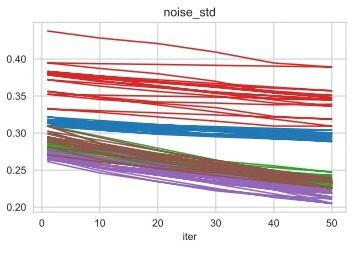
\includegraphics[width=0.5\textwidth]{imagenes/conv1_noise.jpg}
	\caption{Convergencia de noise.}
	\label{fig:conv1_noise}
\end{figure}


En el eje 'x' de cada cuadro se puede el número de iteración al que corresponde cada medida aproximada, mientras que en el eje 'y' se observa el valor del parámetro correspondiente. Los valores correspondientes a variable medida del paciente se gráfica con un color distinto en el caso de \textit{g}, \textit{v0} y \textit{noise}.Hay seis colores diferentes en cada una de estas gráfica, ya que se ha hecho el estudio para seis marcadores distintos: ABETA, HVLTRDLY, LNS, MEANCAU, SDMT y SFT. Por otra parte, cada linea representa las estimaciones de cada uno de los 10 modelos generados.\\

\subsection{Curvas características individuales}
Por otro lado, se gráfican las trayectorias \textit{'short-term'} que representan la estimación de la progresión de cada uno de los marcadores del paciente escogido.\\

El programa genera dos conjunto de seis cuadros para cada uno de los 10 modelos, siendo cada cuadro la estimación de los valores de una variable y el primer conjunto grafica los números normalizados de las mismas y el segundo en escala original. Es decir, se obtienen un total de veinte conjuntos con seis gráficas en su interior, ya que se trabaja con un bootstrap de valor 10, lo que indica que se generan 10 modelos. \\

Además de representarse en cada cuadro la curva estimada, se indican los valores de cada variable en cada observación del paciente con un punto, para así poder ver cuan precisa es la estimación de la trayectoria a corto plazo.\\

De manera ilustrativa, en este documento se muestran las gráficas dibujadas para el modelo número cinco,  viendo en primer lugar los valores normalizados para las seis variables escogidas en la imagen\ref{fig:trayM5norm} y después las curvas para los valores originales en la figura \ref{fig:trayM5orig}.\\

\begin{figure}[t]
	\centering
	\includegraphics[width=1\textwidth]{imagenes/trajectory\_norm\_plot\_model\_5.png}
	\caption{Trayectoria Normalizada del modelo 5.}
	\label{fig:trayM5norm}
\end{figure}

\begin{figure}[t]
	\centering
	\includegraphics[width=1\textwidth]{imagenes/trajectory\_orig\_plot\_model\_5.png}
	\caption{Trayectoria original del modelo 5.}
	\label{fig:trayM5orig}
\end{figure}

El resto de representaciones se pueden encontrar en la siguiente ruta del proyecto:
\begin{center}
		\texttt{Demos/rroca\_python/pred\_sujeto/\\
		plots/norm\_orig}. 
\end{center}


\section{Modelos de progresión con múltiples sujetos}
Como resultados se obtienen los parámetros correspondientes a las prestaciones de los DPMs. Con ellos se podrán comparar, entre los distintos modelos estimados,las predicciones tanto de la progresión de la enfermedad en los distintos pacientes, como el pronóstico estimado y el estado cognitivo de los mismos \cite{ghazi2021robust}. El objetivo de esto es encontrar la combinación de biomarcadores que sirva para predecir el avance de la enfermedad y pronosticar el declive cognitivo de una forma más precisa y eficaz. \\

Todas las métricas calculadas con este propósito se ubican en el directorio:
\begin{center}
	\texttt{/home/rroca/demo/multi\_leaspy/outputs/prestaciones}
\end{center}

Para cada DPM se genera una carpeta llamada \texttt{Leaspy\_vars\_} seguido de los índices de los marcadores escogidos para ese modelo (por ejemplo: \texttt{5\_10\_11}). En ellas se guardan distintos Excels para guardar los valores del MAE y NMAE para los grupos de \textit{train} y de \textit{test}. También contienen archivos .NPY con las puntuaciones de progresión de la enfermedad (DPS) para los dos conjuntos de individuos, y así poder cargar los valores desde el programa si fuera necesario. Por último también se crean dos hojas de cálculo donde se almacenará la media del MAE y del NMAE del modelo concreto y la media de área bajo la curva y los distintos tiempos de conversión y la reserva cognitiva. Esto valores, además de guardarse dentro de cada carpeta por separado, se van añadiendo a dos Excels generales, llamados \texttt{PRESTACIONES\_GENERALES\_MAE.xlsx} y \texttt{PRESTACIONES\_GENERALES\_diag.xlsx} donde cada fila recoge la media de las métricas para los modelos que se van estimando. Estos dos ficheros se ubican directamente en la carpeta:
\begin{center}
	\texttt{/home/rroca/demo/multi\_leaspy/outputs/prestaciones}
\end{center}


\subsection{Evaluación de las trayectorias estimadas}
Para comprobar la rigurosidad de las trayectorias \textit{short-term} estimadas, se implementa la estimación del NMAE. Para cada modelo, es la media de la diferencias entre las estimaciones en escala normalizada y las muestras en cada tiempo muestreado. Cada una de las variables obtiene valor de un NMAE.\\

Además, se consiguió realizar la interpolación inversa de los valores para obtener el error medio absoluto (MAE) en la escala original de cada biomarcador. Se calculó la media para el conjunto de pacientes tanto de entrenamiento como de test para cada uno de los bootstraps y para cada una de las variables de cada modelo estimado. Por ejemplo, para el modelo formado por los marcadores MOCA, LNS y SFT (con índices 1,5 y 10) se obtienen las tablas de las figuras \ref{tabla_MAE_train} y \ref{tabla_MAE_test} para el MAE de \textit{train} y de \textit{test}. \\

\begin{table}[h!]
	\centering
	\begin{tabular}{|c|c|c|c|}
		\hline
		btstrp & \textbf{moca} & \textbf{lns} & \textbf{sft} \\ \hline
		0 & 1.6582 & 1.4737 & 7.8544 \\ \hline
		1 & 1.7160 & 1.4912 & 7.3873 \\ \hline
		2 & 1.6892 & 1.5227 & 7.7018 \\ \hline
		3 & 1.6896 & 1.5120 & 7.3432 \\ \hline
		4 & 1.6656 & 1.5622 & 7.6081 \\ \hline
		5 & 1.6865 & 1.5595 & 7.5482 \\ \hline
		6 & 1.6567 & 1.5500 & 7.5810 \\ \hline
		7 & 1.6903 & 1.5761 & 7.5575 \\ \hline
		8 & 1.7050 & 1.5848 & 7.4854 \\ \hline
		9 & 1.6774 & 1.5873 & 7.5820 \\ \hline
	\end{tabular}
	\caption{MAE de los diez \textit{bootstraps} para MOCA, LNS y SFT para los pacientes de entrenamiento.}
	\label{tabla_MAE_train}
\end{table}

\begin{table}[h!]
	\centering
	\begin{tabular}{|c|c|c|c|}
		\hline
		btstrp & \textbf{moca} & \textbf{lns} & \textbf{sft} \\ \hline
		0 & 1.7401 & 1.4582 & 6.7184 \\ \hline
		1 & 1.8033 & 1.4592 & 6.3295 \\ \hline
		2 & 1.7849 & 1.4951 & 6.6530 \\ \hline
		3 & 1.7797 & 1.4815 & 6.3722 \\ \hline
		4 & 1.7444 & 1.5166 & 6.5898 \\ \hline
		5 & 1.8134 & 1.5225 & 6.6369 \\ \hline
		6 & 1.7344 & 1.4912 & 6.6888 \\ \hline
		7 & 1.7944 & 1.5486 & 6.6537 \\ \hline
		8 & 1.8161 & 1.5529 & 6.5911 \\ \hline
		9 & 1.8219 & 1.5663 & 6.6685 \\ \hline
	\end{tabular}
	\caption{MAE de los diez \textit{bootstraps} paralos biomarcadores MOCA, LNS y SFT para los pacientes de prueba.}
	\label{tabla_MAE_test}
\end{table}

Además de las tablas generadas para visualizar el MAE y el NMAE de cada modelo, se genera un Excel llamado \texttt{PRESTACIONES\_GENERALES\_MAE} donde se van añadiendo las medias del error medio absoluto y del error medio absoluto normalizado para cada modelo estimado. Esto permite comparar la precisión de la trayectoria \textit{short-term} estimada para cada uno, visualizando la tabla de la figura \ref{tab:nmae_mae_resultados}.

\begin{table}[t]
	\centering
	\begin{tabular}{|c|c|c|c|c|}
		\hline
		\textbf{\scriptsize{INDEX}} & \textbf{\scriptsize{NMAE\_train}} & \textbf{\scriptsize{NMAE\_test}} & \textbf{\scriptsize{MAE\_train}} & \textbf{\scriptsize{MAE\_test}} \\ \hline
		2\_11\_16 & 0.154 & 0.148 & 1.337 & 1.267 \\ 
		& 0.143 & 0.158 & 4.828 & 4.740 \\ 
		& 0.103 & 0.094 & 235.426 & 219.423 \\ \hline
		1\_2\_4   & 0.187 & 0.181 & 1.965 & 2.065 \\ 
		& 0.249 & 0.245 & 1.896 & 1.854 \\ 
		& 0.247 & 0.237 & 2.273 & 2.206 \\ \hline
		10\_11\_15& 0.101 & 0.101 & 4.787 & 4.455 \\ 
		& 0.141 & 0.158 & 4.965 & 4.749 \\ 
		& 0.094 & 0.094 & 133.853 & 139.667 \\ \hline
		...  & ... & ... & ... & ...\\ \hline
	\end{tabular}
	\caption{Métricas NMAE y MAE para los modelos considerados.}
	\label{tab:nmae_mae_resultados}
\end{table}




\subsection{Clasificación del estado clínico}
Para clasificar el estado cognitivo se utiliza  un clasificador bayesiano basado en el 'Disease Progresion Score'(DPS)($s_{ij}$) y que utiliza un kernel de estimación de la densidad (KDE) basado en estimaciones acordes.
\begin{equation}
	s_{ij}=\alpha_{i}t_{ij}+\beta_{i}
\end{equation}

 Para medir la fiabilidad de la probabilidad a posteriori de desarrollo del declive cognitivo se utiliza como parámetro el Área Bajo la Curva (AUC).Esto mide la precisión del modelo de determinar la aparición del deterioro cognitivo comparándolo con las etiquetas (\textit{CN} o \textit{MCI}) de los pacientes en cada una de las visitas.\\
 
 Un AUC más cercano a 1 indica que el las predicciones realizadas por el modelo son fiables. Por lo que con los resultados obtenidos se esperan encontrar valores mas cercanos a 1 que a 0,5. Para conseguir un modelo robusto, se calcula un Area Bajo la Curva para cada \textit{bootstrap} y luego se calcula la media. Este valor se guarda tanto en un archivo \texttt{.xlsx} dentro del directorio de \texttt{prestaciones} en una carpeta que indique el modelo evaluado, como en el excel general donde se van guardando todas las metricas, el cual se encuentra en el directorio:

 \begin{center}
 	\texttt{/home/rroca/demo/multi\_leaspy/outputs/prestaciones
 		/PRESTACIONES\_GENERAL\_diag.xlsx}
 \end{center}

Otro indicador de la exactitud de los modelo son los parámetros \textbf{percentage\_PD\_CU} y \textbf{percentage\_PD\_MCI}. Estos se encuentran en el archivo del directorio:
\begin{center}
	\texttt{/home/rroca/demo/multi\_leaspy/outputs/prestaciones
		/PRESTACIONES\_GENERAL\_diag.xlsx}
\end{center}
en las columnas con los mismos nombres y con el indicador de diferenciación del grupo de \textit{train} y de \textit{test}. \\

Estas métricas miden el rendimiento de los modelos para predecir el inicio dela conversión a deterioro cognitivo leve (MCI) a partir de los datos de los sujetos. Por un lado mide el porcentaje de pacientes que predice correctamente como convertidos a MCI y lo guarda en las columnas \textbf{perc\_PD\_MCI\_test} y \textbf{perc\_PD\_MCI\_train}. Por otro lado, se calcula el porcentaje de sujetos que el modelo predice correctamente como sanos (CU) y los registra en las columnas con nombre \textbf{perc\_PD\_CU\_test} y \textbf{perc\_PD\_CU\_train}. 




\subsection{Medidas relacionadas con los plazos de conversión hacia el declive cognitivo}

Por último, se calculan las correlaciones de los tiempos de conversión hacia el declive cognitivo de los individuos de entrenamiento y de prueba, y también de la reserva cognitiva de ambos grupos. Estos medidores indican, por un lado la precisión a la hora de predecir a que edad convierten los pacientes, y por otro lado la exactitud del cálculo de años de reserva que les quedan antes de entrar en la fase de deterioro cognitivo. \\

Se calculan estos dos parámetros ya que no es lo mismo comparar las edades estimadas, que los años de reserva. En el primer caso como la escala es mucho mayor aunque el modelo tenga un error a la hora de predecir de un par de años, la correlación variaría en unas décimas. Mientras que en el caso de la reserva cognitiva, una diferencia de dos años puede suponer un que el índice pase de un 0,7 de precisión a un 0,2. Por lo que los parámetros de la reserva cognitiva nos da un valor más exacto de cuan fiable es el modelo.\\

Estas medidas, al igual que la del Área Bajo la Curva (AUC) se guardan en el excel del directorio:

\begin{center}
	\texttt{/home/rroca/demo/multi\_leaspy/outputs/prestaciones
		/PRESTACIONES\_GENERAL\_diag.xlsx}
\end{center}

Más concretamente en las cuatro columnas con los siguientes nombres:
\begin{itemize}
	\item \textbf{corr\_PD\_MCI\_reserve\_train} y \textbf{corr\_PD\_MCI\_reserve\_test}: medidas de la correlación entre la reserva cognitiva real y la estimada para \textit{train} y \textit{test}
	\item \textbf{corr\_PD\_MCI\_age\_train} y \textbf{corr\_PD\_MCI\_age\_test}: parámetrso para la correlación entre las edades de conversión reales y las estimadas para los individuos de entrenamientos y de prueba.
\end{itemize}

En la figura \ref{tab:resultados_biomarcadores} se muestran las medidas de algunos de los modelos estimados y guardados en el fichero \texttt{PRESTACIONES\_GENERAL\_diag.xlsx}. Para referirse a la medidas tomadas para el grupo de entrenamiento se adjunta un 1 al final del nombre de las columnas, y para referirse al grupo de prueba se adjunta un 2.


\begin{table}[H]
	\centering
	\begin{adjustbox}{max width=\textwidth}
		\begin{tabular}{|c|c|c|c|c|c|c|c|c|c|c|}
			\hline
			\rotatebox{90}{\scriptsize{\textbf{INDEX}}} & \rotatebox{90}{\scriptsize{\textbf{AUC\_1}}} & \rotatebox{90}{\scriptsize{\textbf{AUC\_2}}} & \rotatebox{90}{\scriptsize{\textbf{perc\_PD\_CU\_2}}} & \rotatebox{90}{\scriptsize{\textbf{perc\_PD\_MCI\_2}}} & \rotatebox{90}{\scriptsize{\textbf{corr\_PD\_MCI\_age\_2}}} & \rotatebox{90}{\scriptsize{\textbf{corr\_PD\_MCI\_reserve\_2}}} & \rotatebox{90}{\scriptsize{\textbf{perc\_PD\_CU\_1}}} & \rotatebox{90}{\scriptsize{\textbf{perc\_PD\_MCI\_1}}} & \rotatebox{90}{\scriptsize{\textbf{corr\_PD\_MCI\_age\_1}}} & \rotatebox{90}{\scriptsize{\textbf{corr\_PD\_MCI\_reserve\_1}}} \\ \hline
			1\_5\_14       & 0.797 & 0.800 & 94.737 & 26.087 & 0.979 & 0.011 & 98.971 & 25.789 & 0.970 & 0.505 \\ \hline
			4\_5\_14\_16   & 0.738 & 0.787 & 98.246 & 14.783 & 0.932 & 0.389 & 98.025 & 16.316 & 0.968 & 0.420 \\ \hline
			1\_5\_10\_18   & 0.789 & 0.796 & 95.088 & 16.522 & 0.960 & 0.489 & 98.683 & 22.237 & 0.983 & 0.579 \\ \hline
			5\_10\_11\_14  & 0.786 & 0.824 & 96.140 & 27.391 & 0.957 & 0.504 & 96.831 & 25.658 & 0.973 & 0.356 \\ \hline
			...  & ... & ... & ... & ... & ... & ... & ... & ... & ... & ... \\ \hline
		\end{tabular}
	\end{adjustbox}
	\caption{Métricas de evaluación clínica para diferentes modelos.}
	\label{tab:resultados_biomarcadores}
\end{table}


\section{Análisis masivo: \textit{multi\_Leaspy} y\textit{ multi\_RPDPM}}
Una vez obtenidas las medidas de distintos conjuntos de biomarcadores, se comparan entre los dos métodos de predicción utilizados: Leaspy y RPDPM. Cabe destacar la preferencia de vectores de menor dimensión, ya que implicarían un menor número de observaciones y de medidas a tomar en los pacientes para poder predecir el avance de la enfermedad, y por lo tanto un menor coste. \\

Para comparar la precisión de los distintos modelos, se tomó como medida de referencia la multiplicación de la detección de pacientes cognitivamente normales (\textbf{perc\_PD\_CU}) por la correlación con la reserva cognitiva (\textbf{corr\_PD\_MCI\_reserve}). En las tablas \ref{tab:RPDPM3} y \ref{tab:RPDPM4y5} se muestran los resultados de los vectores de características que mejores puntuaciones han mostrado para el método RPDPM en las medidas de detección de sujetos cognitivamente normales y con declive cognitivo leve, y en las correlaciones de la edad y de la reserva cognitiva. En el primer caso se muestran vectores de menor dimensión, mejores para aplicaciones clínicas ya que solo haría falta observar tres biomarcadores, y en el segundo caso para combinaciones de mayor tamaño. En las tablas \ref{tab:LEASPY3} y \ref{tab:LEASPY4y5} se muestran los vectores con mejores resultados para el caso de Leaspy, dividiendo las tablas también en función del numero de características de las combinaciones.

A continuación, se muestran los vectores de marcadores que mejores resultados han dado tanto en Leaspy como en RPDPM, en función de la cantidad de variables utilizadas. 

\subsection{Leaspy}
Para el método de Leaspy, el vector de menor dimensión que mejores resultados a mostrado es el formado por los biomarcadores:
\begin{center}
	\textbf{\{updrs\_totscore, tau y asyn\}}
\end{center}
En cuanto a los vectores de dimensiones mayores (cuatro o cinco biomarcadores), que mejores resultados han dado en las métricas de calidad de detección del estado de los pacientes y de la aparición del declive cognitivo son los siguientes:
\begin{center}
	\textbf{\{updrs3\_score\_on, updrs\_totscore\_on, ptau, asyn\}}		
\end{center}
\begin{center}
	\textbf{\{updrs3\_score\_on, updrs2\_score, ptau, mean\_caudate, mean\_putamen\}}
\end{center}

Estos tres vectores muestran las siguientes puntuaciones en las medidas de detección de pacientes PD\_CU en el grupo de \textit{test}: 100, 98.24 y 97.36. Y sus valores en la correlación con la reserva cognitiva es 1 en los tres casos. \\

Dado que los valores son prácticamente iguales para las tres combinaciones, el más  conveniente para la práctica clínica es el de menor dimensión como ya se explicó previamente. \\

\subsection{RPDPM}
Para el caso de RPDPM desarrollado en MATLAB, los vectores que mejores resultados mostraron con dimensiones de 5, 4 y 3 biomarcadores fueron:

\begin{center}
	\textbf{\{GDS, UPSIT, REM, LNS, ADL\}}		
\end{center}
\begin{center}
	\textbf{\{UPSIT, LNS, SDMT, ADL\}}
\end{center}
\begin{center}
	\textbf{\{SDMT, JLO, HVLTRDLY\}}
\end{center}

De estos tres, el que mejores puntuaciones muestra es al mismo tiempo el de menor dimensión, por lo que la combinación de biomarcadores formada por SDMT, JLO y HVLTRDLY también es el más apropiado para la aplicación clínica. Los valores de estos tres vectores en cuanto a la detección de pacientes PD\_CU son respectivamente: 97.75, 97.46 y 98.92. Y los valores de la correlación de la reserva cognitiva para los pacientes de test para esas combinaciones son: 0.432, 0.654 y 0.725.\\

\begin{table}[H]
	\centering
	\begin{adjustbox}{max width=\textwidth}
		\begin{tabular}{|c|c|c|c|c|c|}
			\hline
			\textbf{BIOMARCADORES} & \textbf{\%PD\_CU} & \textbf{\%PD\_MCI} & \textbf{corr\_PD\_MCI\_edad} & \textbf{corr\_PD\_MCI\_reserva} & \textbf{AUC} \\ \hline
			U, L, S, A  & 97.46 & 32.47 & 0.978 & 0.654 & 0.803 \\ \hline
			U, L, S, M  & 97.33 & 28.52 & 0.968 & 0.551 & 0.790 \\ \hline
			S, J, H, M & 98.75 & 30 & 0.973 & 0.684 & 0.794 \\ \hline
			G, L, S, A  & 97.58 & 36.67 & 0.980 & 0.613 & 0.813 \\ \hline
			G, U, R, L, A & 97.75 & 39.63 & 0.982 & 0.432 & 0.833 \\ \hline
		\end{tabular}
	\end{adjustbox}
	\caption{Mejores combinaciones de biomarcadores de mayor dimensión con 4 o 5 características para el método de RPDPM, basado en las medidas de la detección de PD\_CU (\%PD\_CU), detección de PD\_MCI (\%PD\_MCI), correlación con la edad (corr\_PD\_MCI\_edad), correlación con la reserva (corr\_PD\_MCI\_reserva) y Área Bajo la Curva (AUC). U=UPSIT, L=LNS, S=SDMT, A=ADL, M=MEANPUT, J=JLO, H=HVLTRDLY, G=GDS, R=REM.}
	\label{tab:RPDPM4y5}
\end{table}

\begin{table}[H]
	\centering
	\begin{adjustbox}{max width=\textwidth}
		\begin{tabular}{|c|c|c|c|c|c|}
			\hline
			\textbf{BIOMARCADORES} & \textbf{\%PD\_CU} & \textbf{\%PD\_MCI} & \textbf{corr\_PD\_MCI\_edad} & \textbf{corr\_PD\_MCI\_reserva} & \textbf{AUC} \\ \hline
			S, J, H  & 98.92 & 29.75 & 0.977 & 0.726 & 0.795 \\ \hline
			L, S, A & 96.63 & 36.05 & 0.975 & 0.584 & 0.795 \\
			\hline
			G, L, J & 98.46 & 36.91 & 0.986 & 0.564 & 0.820 \\
			\hline
			G, L, S & 97.21 & 38.64 & 0.980 & 0.520 & 0.803 \\ \hline
			J, H, SF & 98.92 & 28.77 & 0.982 & 0.564 & 0.817 \\   \hline
		\end{tabular}
	\end{adjustbox}
	\caption{Mejores combinaciones de biomarcadores de menor dimensión con 3 características para el método de RPDPM, basado en las medidas de la detección de PD\_CU (\%PD\_CU), detección de PD\_MCI (\%PD\_MCI), correlación con la edad (corr\_PD\_MCI\_edad), correlación con la reserva (corr\_PD\_MCI\_reserva) y Área Bajo la Curva (AUC). S=SDMT, J=JLO, H=HVLTRDLY, L=LNS, A=ADL, G=GDS, SF=SFT.}
	\label{tab:RPDPM3}
\end{table}


\begin{table}[H]
	\centering
	\begin{adjustbox}{max width=\textwidth}
		\begin{tabular}{|c|c|c|c|c|c|}
			\hline
			\textbf{BIOMARCADORES} & \textbf{\%PD\_CU} & \textbf{\%PD\_MCI} & \textbf{corr\_PD\_MCI\_edad} & \textbf{corr\_PD\_MCI\_reserva} & \textbf{AUC} \\ \hline
			 U3O, UTO, P, A & 98.25 & 1.74 & 1.00 & 1.00 & 0.696\\ \hline
			 SC, M, B, S & 100 & 12.17 & 0.997 & 0.881 & 0.815\\ \hline
			 U3O, U3, U2, UTO & 98.60 & 6.52 & 0.996 & 0.908 & 0.730 \\ \hline
			 U3O, U2, P, MC, MP  & 97.37 & 3.48 & 1.00 & 1.00 & 0.769\\ \hline
			 SC, M, SF, HI, R & 98.77 & 8.69 & 1.00 & 1.00 & 0.811\\ \hline
		\end{tabular}
	\end{adjustbox}	
	\caption{Mejores combinaciones de biomarcadores de mayor dimensión con 4 o 5 características para el método de Leaspy, basado en las medidas de la detección de PD\_CU (\%PD\_CU), detección de PD\_MCI (\%PD\_MCI), correlación con la edad (corr\_PD\_MCI\_edad), correlación con la reserva (corr\_PD\_MCI\_reserva) y Área Bajo la Curva (AUC). U3O=UPDRS3\_SCORE\_ON, UTO=UPDRS\_TOTSCORE\_ON, P=PTAU, A=ASYN, SC=SCOPA, M=MSEADLG, B=BJLOT, S=SDMT, U3=UPDRS3\_SCORE, U2=UPDRS2\_SCORE, MC=MEAN\_CAUDATE, MP=MEAN\_PUTAMEN, SF=SFT, HI=HVLT\_INMEDIATERECALL, R=REM.}
	\label{tab:LEASPY4y5}
\end{table}



\begin{table}[H]
	\centering
	\begin{adjustbox}{max width=\textwidth}
		\begin{tabular}{|c|c|c|c|c|c|}
			\hline
			\textbf{BIOMARCADORES} & \textbf{\%PD\_CU} & \textbf{\%PD\_MCI} & \textbf{corr\_age\_MCI} & \textbf{corr\_reserve\_MCI} & \textbf{AUC} \\ \hline
			UT, T, A & 100 & 6.96 & 1.00 & 1.00 & 0.723 \\ \hline
			UTO, T, A & 99.83 & 10.00 & 0.970 & 0.927 & 0.725 \\ \hline
			UTO, P, A & 99.83 & 8.26 & 1.00 & 1.00 & 0.724 \\ \hline
			U2, UTO, AB & 100 & 3.48 & 1.00 & 1.00 & 0.718 \\ \hline
			SC, H, R & 100 & 6.52 & 1.00 & 1.00 & 0.74 \\ \hline
		\end{tabular}
	\end{adjustbox}
	\caption{Mejores combinaciones de biomarcadores de menor dimensión con 3 características, basadas en las medidas de la detección de PD\_CU (\%PD\_CU), detección de PD\_MCI (\%PD\_MCI), correlación con la edad (corr\_age\_MCI), correlación con la reserva (corr\_reserve\_MCI) y Área Bajo la Curva (AUC). UT=UPDRS\_TOTSCORE, T=TAU, A=ASYN, UTO=UPDRS\_TOTSCORE\_ON, P=PTAU, U2=UPDRS2\_SCORE, AB=ABETA, SC=SCOPA, H=HVLTRDLY, R=REM.}
	\label{tab:LEASPY3}
\end{table}

